% !TEX options=--shell-escape
\documentclass[usenames,dvipsnames,9pt]{beamer}
\usetheme{metropolis}

% Not working in Overleaf
% \makeatletter
% \def\input@path{{../support/beamer-template/}}
% \makeatother
% \usepackage{../support/beamer-template/beamerthememetropolis}

\usepackage[utf8]{inputenc}
\usepackage[czech]{babel}
\selectlanguage{czech}

\usepackage{hyperref}
\usepackage{fontawesome}
\usepackage{minted}
\usepackage{mathtools}
\usepackage{tabularx}
\usepackage{smartdiagram}
\usepackage{amssymb}
\usepackage{qrcode}

% Commands shared between most of the tutorial slides

% Homework deadlines
\newcommand{\hwVIIdeadline}{10. 5. 2020}



% Download icon and text with link relative to the root of the courseware site
\newcommand{\download}[1]{\hfill\faDownload\hspace{5pt}\href{https://cw.fel.cvut.cz/wiki/_media/courses/be4m36mas/#1}{\tt #1}\\[1.3em]}

% Draw eye icon
\newcommand{\see}[1]{\faEye\hspace{5pt}#1}

\newcommand{\sep}{\hspace{10pt}/\hspace{10pt}}

\def\Ipe#1{\def\IPEfile{#1}\input{#1}}

% Draw pacman icon
\newcommand{\pacman}[1]{\tikz[baseline=.1em,scale=.6]{
    \useasboundingbox (.02,0) rectangle (.6,.6);
  \draw [fill=#1] (.3,.3) -- ++(25:.3) arc (+25:+335:.3) -- cycle;

}}

% Draw ghost icon
\newcommand{\ghost}[1]{\tikz[baseline=.1em,scale=.5]{
  \draw [fill=#1] (0,0) -- (0,.5) arc (+180:0:.3) -- (.6,0) --
  (.5,.15) -- (.4,0) -- (.3,.15) -- (.2,0) -- (.1,.15) -- cycle;
    \coordinate (eye) at (360*rand:.03);
    \foreach \x in {.17,.43}{
      \fill[white] (\x,.5) circle[radius=.1];
      \fill[black] (\x,.5) ++(eye) circle[radius=.05];
    }
}}

\newcommand{\desc}[2]{
  #1

  \vspace{-0.6em}
  \hfill\begin{minipage}{0.9\linewidth}
    #2
  \end{minipage}

  \vspace{0.2em}
}

\newcommand{\redc}{\tikz\draw[red,fill=red] (0,0) circle (.5ex);}

\newcommand{\greenc}{\tikz\draw[green,fill=green] (0,0) circle (.5ex);}


% Default url for generating QR code with feedback form.
\newcommand{\defaultfeedbackurl}{https://forms.gle/vwbWazEu14w1Kf487}

% Generate frame with QR code to a feedback form.
\newcommand{\framefeedback}[1][\defaultfeedbackurl]{
  \begin{frame}[standout]
    \begin{minipage}{0.4\linewidth}
      \begin{center}
        \textbf{\LARGE Díky za pozornost!}
      \end{center}

      \vspace{3em}

      \raggedleft\small Budeme rádi za Vaši\\zpětnou vazbu! $\rightarrow$
    \end{minipage}
    \hfill
    \begin{minipage}{0.5\linewidth}
      \vspace{4em}
      \centering\qrcode[height=\linewidth]{#1}\\
      \vspace{0.8em}
      \url{#1}
    \end{minipage}
  \end{frame}
}

\title{Vlákna a přístup ke sdílené paměti}
%\subtitle{Organizace předmětu a seznámení se s paralelizací}
\date{}
\institute{B4B36PDV -- Paralelní a distribuované výpočty}

\metroset{block=fill}

\begin{document}
\maketitle

\begin{frame}
  Minulé cvičení:
  \vspace{-2.8em}
  \begin{center}
    \Large\emph{``Paralelizace nám může pomoct...''}
  \end{center}
  \pause
  \vspace{1.5em}
  B4B36PDV:
  \vspace{-2.8em}
  \begin{center}
    \Large\emph{``Ale ne všechny přístupy vedou\\ke stejně dobrým výsledkům!''}
  \end{center}
  \pause
  \vspace{2.5em}
  Dnešní menu: \hspace{10pt} \huge Vlákna a jejich synchronizace
\end{frame}

\begin{frame}
  \frametitle{Osnova}
  \begin{itemize}
    \item Opakování z minulého cvičení
    \item Vlákna v C++ 11
    \item Přístup ke sdílené paměti a synchronizace\\[1.5em]
    \item Zadání první domácí úlohy
  \end{itemize}
\end{frame}

%\begin{frame}[standout]
%  \begin{minipage}{0.4\linewidth}
%    \begin{center}
%      \textbf{\LARGE Jsem tady!}
%    \end{center}
%
%    \vspace{3em}
%
%    \raggedleft\small Označte se! $\rightarrow$
%  \end{minipage}
%  \hfill
%  \begin{minipage}{0.5\linewidth}
%    \vspace{4em}
%    \centering
\includegraphics[width=\linewidth]{figs/qr_feedback.pdf}
%  \end{minipage}
%\end{frame}

\begin{frame}[standout]
  \url{http://goo.gl/a6BEMb}
\end{frame}

% \section{Opakování z minulého cvičení}

% \begin{frame}
%   \frametitle{Moderní procesor}
%   Možné ``nástrahy'' použití moderního procesoru s více jádry a cache:
%   \begin{itemize}
%     \item Komunikace s pamětí je stále pomalá (problém \emph{cache-miss})
%     \item Přístup ke sdíleným datům více vlákny (\emph{true sharing})
%     \item Udržování koherence cache může být drahé (\emph{false sharing}) \\[2em]
%     \item Úloha nemusí být vhodná pro paralelizaci
%   \end{itemize}
% \end{frame}

{\setbeamertemplate{frame footer}{\see{{\tt PDVCrypt.cpp},\ \ \ {\tt decrypt.cpp} \sep {\tt make decrypt}} \hfill \faDownload \hspace{5pt} \texttt{decrypt\_data.zip}}
\begin{frame}[fragile]
  \frametitle{Šifra \texttt{PDVCrypt}}
  Vzpomeňte si na šifru z minulého cvičení
  \begin{center}
    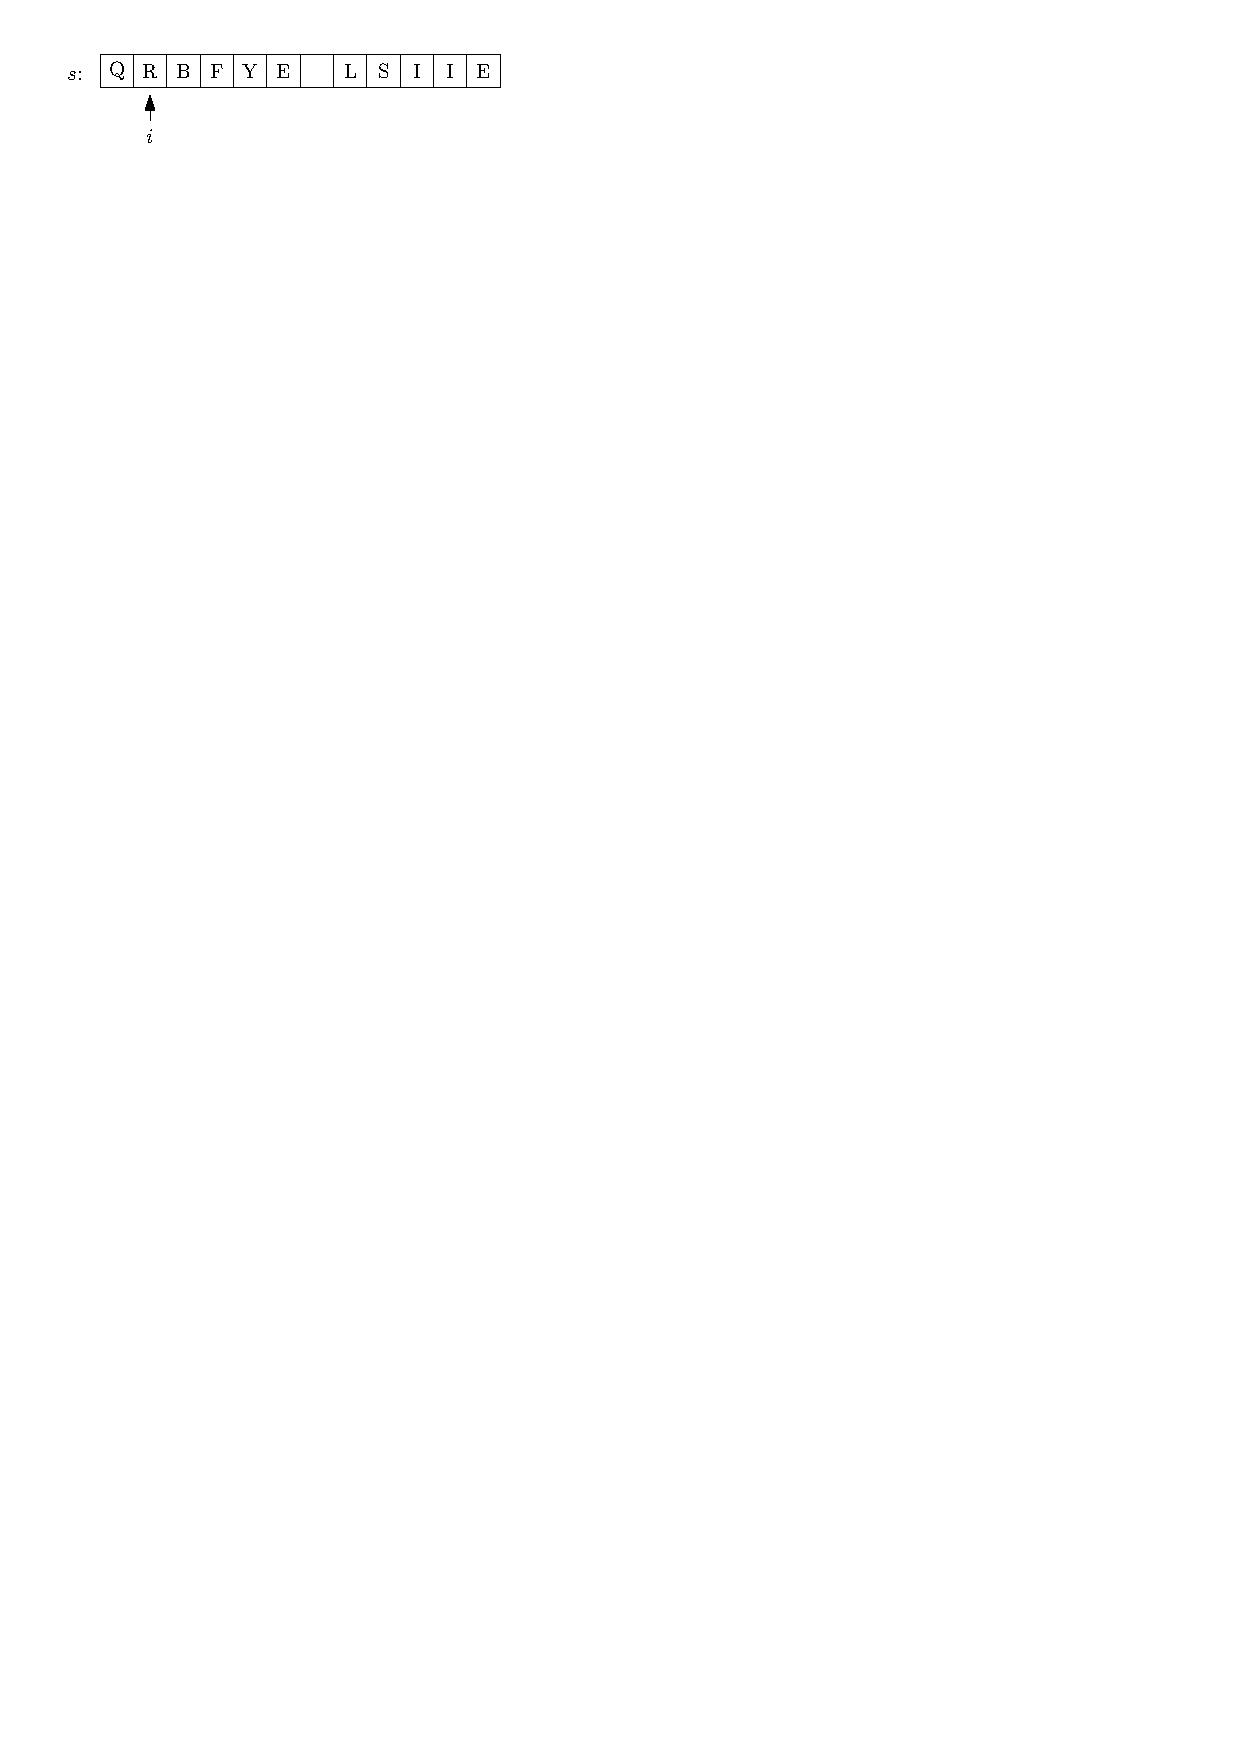
\includegraphics[scale=0.8]{figs/pdvcrypt.pdf}
  \end{center}

  {\small
  Jeden krok dešifrování:
  \vspace{-1em}
  \begin{itemize}
    \item $s_i \gets \Big[ s_i + p_1 \times secret(\overbrace{s_{[i-2 .. i+2]}}^{\text{EQRBF}}) \Big] \ \mathrm{mod}\ |\Sigma|$
    \item $i \gets \Big[ i + p_2 \times secret(s_{[i-2 .. i+2]}) \Big] \ \mathrm{mod} \ |s|$
  \end{itemize}
  ... opakován $N$-krát}

  \vspace{1em}
\end{frame}
}

{\setbeamertemplate{frame footer}{\see{{\tt decryption.cpp},\ \ \ {\tt benchmark.cpp}, \ \ \ {\tt PDVCrypt.cpp} \sep {\tt make benchmark}}}
\begin{frame}[fragile]
  \frametitle{Šifra \texttt{PDVCrypt}}
  Jak vypadala paralelizace v OpenMP?

    \begin{minted}[fontsize=\footnotesize]{c}
void decrypt_openmp(const PDVCrypt &crypt, 
        std::vector<std::pair<std::string, enc_params>> &encrypted,
        unsigned int numThreads) {
    const unsigned long size = encrypted.size();

    #pragma omp parallel for num_threads(numThreads)
    for(unsigned long i = 0 ; i < size ; i++) {
        auto & enc = encrypted[i];
        crypt.decrypt(enc.first, enc.second);
    }
}
    \end{minted}
    
\end{frame}
}

\begin{frame}[fragile]
  \frametitle{Šifra \texttt{PDVCrypt}}
  \begin{minted}{c}
    #pragma omp parallel for num_threads(numThreads)
    for(...) {
      ...
    }
  \end{minted}
  
  \vspace{2em}

  \hfill\Large Co se ve skutečnosti stalo?    
\end{frame}

\section{Vlákna v C++ 11}

\begin{frame}[fragile]
  C++11 (přes \mintinline{c}{#include <thread>}) poskytuje multiplatformní přístup k práci s vlákny:

  \vspace{1em}

  \begin{minted}[fontsize=\small]{c}
    #include <iostream>
    #include <thread>

    void dummy_thread(int id, int n) {
      std::cout << "Thread " << id << " prints " << n << "\n";
    }

    int main() {
      std::thread t1(dummy_thread, 1, 2);
      std::thread t2(dummy_thread, 2, 42);
      t1.join();
      t2.join();

      return 0;
    }
  \end{minted}
\end{frame}

\begin{frame}[fragile]
  \frametitle{Kompaktnější zápis pomocí lambda funkcí}
  \begin{minted}[fontsize=\small]{c}
    #include <iostream>
    #include <thread>

    void dummy_thread(int id, int n) {
      std::cout << "Thread " << id << " prints " << n << "\n";
    }

    std::thread t1(dummy_thread, 1, 2);
    std::thread t2([&] (int id, int n) {
      std::cout << "Thread " << id << " prints " << n << "\n";
    }, 2, 42);
  \end{minted}

  \vspace{1em}\hrule\vspace{1em}

  Lambda funkce (uvozená pomocí \mintinline{c}{[&]}) má navíc přístup ke všem lokálním proměnným.
  \begin{itemize}
    \item Nemusíme si je tak předávat například pointery na lokální proměnné jako argumenty, pokud s nimi chceme pracovat
  \end{itemize}
\end{frame}

% %{\setbeamertemplate{frame footer}{}
% \begin{frame}[fragile]
% Standardní knihovna C++ poskytuje prostředky pro práci s vlákny.
%   \begin{itemize}
%     \item Vlákna jsou exportována hlavičkou \texttt{<thread>}
%         \item Konstruktor vlákna získá prvním argumentem funkci, kterou bude vykonávat, ostatní argumenty předá volané funkci
%     \item Vlákno je nejhrubší jednotka paralelismu
%   \end{itemize}
  
%     \vspace{1em}
%     \pause
    
% %    \begin{minipage}{0.4\linewidth}
% %    
% %        \begin{minted}[fontsize=\footnotesize]{c}
% %int main() {
% %	std::thread t1(function, 1, 2);
% %	t1.join();
% %}
% %    \end{minted}
% %  \end{minipage}
% %  \hfill
% %  \begin{minipage}{0.5\linewidth}
% %      
% %        \begin{minted}[fontsize=\footnotesize]{c}
% %void function(int id, int n) {
% %	std::cout << "vlakno " << id << " rika ahoj\n";
% %}
% %    \end{minted}
% %  \end{minipage}

%         \begin{minted}[fontsize=\footnotesize]{c}
% #include <iostream>
% #include <thread>

% void function(int id, int n) {
% 	std::cout << "Vlakno " << id << " tiskne " << n << "\n";
% }

% int main() {
% 	std::thread t1(function, 1, 2);
% }
%     \end{minted}
  
% \end{frame}

% \begin{frame}[fragile]
% Dříve, než je zavolán destruktor \texttt{std::thread}, musíme
%   \begin{itemize}
%   \item zavolat metodu \texttt{join} -- spouštějící vlákno čeká, než spuštěné
% vlákno doběhne
% \item nebo zavolat metodu \texttt{detach} -- spuštěné vlákno je autonomní
%   \end{itemize}
  
%   \pause
%   \vspace{1em}

%         \begin{minted}[fontsize=\footnotesize]{c}
% #include <iostream>
% #include <thread>

% void function(int id, int n) {
% 	std::cout << "Vlakno " << id << " tiskne " << n << "\n";
% }

% int main() {
% 	std::thread t1(function, 1, 2);
% 	t1.join();
% }
%     \end{minted}
    
% \end{frame}

{\setbeamertemplate{frame footer}{\see{{\tt decryption.cpp},\ \ \ {\tt benchmark.cpp},\ \ \ {\tt PDVCrypt.cpp} \sep {\tt make benchmark}}}
\begin{frame}[fragile]
  \begin{block}{Vyřešte úlohu pomocí vláken}
    Doimplementujte tělo metody \texttt{decrypt\_threads\_1} v souboru \texttt{decryption.cpp}.
    Spusťte \texttt{numThreads} vláken, kdy každé vlákno bude vykonávat funkci \texttt{process}.
  \end{block}

  \pause

  \vspace{2em}
  \begin{center}
    \Large
    Co je na této implementaci špatně?
  \end{center}
\end{frame}
}

% \begin{frame}[fragile]
%   \vspace{1em}
%   \begin{block}{Řešení}
  
%     \begin{minted}[fontsize=\footnotesize]{c}
% void decrypt_threads_1(const PDVCrypt &crypt, 
% 	std::vector<std::pair<std::string, enc_params>> &encrypted) {
%     const unsigned long size = encrypted.size();
%     unsigned long i = 0;
    
%     auto thread_func = [&i]() {
%         while(true) {
%                 if (i >= size) break;
%                 auto & enc = encrypted[i++];
%                 crypt.decrypt(enc.first, enc.second);
%             }
%     };

%     vector<thread> threads;
%     for(unsigned int t = 0 ; t < n_threads ; t++) {
%         threads.emplace_back(thread_func);
%     }
%     for(unsigned int t = 0 ; t < n_threads ; t++) {
%         threads[t].join();
%     }
% }
%     \end{minted}
%       \end{block}
% \end{frame}
% }

% %{\setbeamertemplate{frame footer}{}}
% \begin{frame}
% Vzhledem k tomu, že vlákna sdílejí paměť, je potřeba je {\bf synchronizovat} !
% \end{frame}

\section{Synchronizace vláken při přístupu ke sdílené paměti}

  
%\begin{frame}[fragile]
%\frametitle{Opakování -- naivní paralelizace}
%
%    \begin{minted}[fontsize=\footnotesize]{c}
%    const unsigned long size = encrypted.size();
%
%    #pragma omp parallel for
%    for(unsigned long i = 0 ; i < size ; i++) {
%        auto & enc = encrypted[i];
%        crypt.decrypt(enc.first, enc.second);
%    }
%    \end{minted}
%
%\end{frame}

\begin{frame}[fragile]
  \frametitle{Varianta opravy č.1: Mutex}
  
  Mutex nám umožňuje zabránit více vláknům využívat stejný zdroj současně.
  \begin{itemize}
    \item Mutex vlastní vždy pouze jedno vlákno a ostatní vlákna musí čekat (mutex = \emph{mutually-exclusive}) \\[0.7em]
    \pause
    \item Můžeme tak naimplementovat kritickou sekci, kam může vstoupit jediné vlákno. V této sekci:
          \begin{itemize}
            \item Zjistíme index, který máme zpracovat
            \item Inkrementujeme hodnotu \texttt{i}
          \end{itemize}
  \end{itemize}

  \pause
  \vspace{1em}

  \begin{minted}[fontsize=\footnotesize]{c}
    #include <iostream>
    #include <thread>
    #include <mutex>

    std::mutex m;
    void dummy_thread() {
      std::cout << "Zde muze byt soucasne vice vlaken." << std::endl;
      {
        std::unique_lock<std::mutex> lock(m);
        std::cout << "Ale zde budu uplne sam..." << std::endl;
      }
      std::cout << "A tady opet nemusim byt sam...";
    }
  \end{minted}

%    \begin{minted}[fontsize=\footnotesize]{c}
%    const unsigned long size = encrypted.size();
%
%    #pragma omp parallel for
%    for(unsigned long i = 0 ; i < size ; i++) {
%        auto & enc = encrypted[i];
%        crypt.decrypt(enc.first, enc.second);
%    }
%    \end{minted}

\end{frame}

%  \begin{frame}
%  \frametitle{Implementace mutexu}
%  
%    \begin{itemize}
%\item Zamykající objekt
%\item Zamýkaný objekt
%\end{itemize}



%\end{frame}

{\setbeamertemplate{frame footer}{\see{{\tt decryption.cpp},\ \ \ {\tt benchmark.cpp},\ \ \ {\tt PDVCrypt.cpp} \sep {\tt make benchmark}}}
\begin{frame}[fragile]
  \frametitle{Varianta opravy č.1: Mutex}
  
  \vspace{1em}
  \begin{block}{Doplňte mutex}
    Opravte metodu \texttt{decrypt\_threads\_1} za použití mutexu.
    Metodu \texttt{decrypt\_threads\_1} neupravujte, opravený kód zapište do metody \texttt{decrypt\_threads\_2}.
  \end{block}
\end{frame}
}

\begin{frame}
  \frametitle{Varianta opravy č.1: Mutex}
  {\Large \faWarning \hspace{10pt} \textbf{Pozor!}}
  
  Použití mutexů skrývá hrozbu \emph{dead-locků}.
  Kód musíme navrhovat tak, aby bylo garantované, že vlákno někdy mutex získá (a provede tak kritickou sekci).
  Jinak zůstane čekat navěky...
\end{frame}

\begin{frame}[fragile]
  \frametitle{Varianta opravy č.2: Atomická proměnná}
  Pokud nám stačí v rámci kritické sekce provést \emph{jednu} operaci nad \emph{jednou} proměnnou, můžeme si vystačit s atomickou operací.
  
  \vspace{1em}

  Příklady atomických operací:
  \begin{itemize}
    \item Inkrementování proměnné typu \mintinline{c}{int}
    \item Vynásobení proměnné typu \mintinline{c}{int} konstantou
  \end{itemize}

  \pause

  \vspace{1em}
  \hrule
  \vspace{1em}

  Jak na to v C++11: \hspace{10pt} \mintinline{c}{#include <atomic>}
  \begin{center}
    \mintinline{c}{int x = 0;}
    \hspace{20pt}$\rightarrow$\hspace{20pt}
    \mintinline{c}{std::atomic<int> x { 0 };}
  \end{center}
\end{frame}

{\setbeamertemplate{frame footer}{\see{{\tt decryption.cpp},\ \ \ {\tt benchmark.cpp},\ \ \ {\tt PDVCrypt.cpp} \sep {\tt make benchmark}}}
\begin{frame}[fragile]
  \frametitle{Varianta opravy č.2: Atomická proměnná}
  
  \vspace{1em}
  \begin{block}{Nahraďte mutex atomickou proměnnou}
    Nahraďte mutex v \texttt{decrypt\_threads\_2} atomickou proměnnou.
    Nový kód zapište do funkce \texttt{decrypt\_threads\_3}.
  \end{block}
\end{frame}
}

% %{\setbeamertemplate{frame footer}{}}
% \begin{frame}[fragile,t]
% %\frametitle{Podmínkové proměnné}
%   \vspace{1em}
%   \begin{block}{Jaký je problém následujícího programu?}

%       \begin{minted}[fontsize=\footnotesize]{c}
% int main() {
%     std::mutex m1; std::mutex m2;
 
%     std::thread t1([&m1, &m2](){
%         for (int i = 0; i < 1000000; ++i) {
%             std::unique_lock<std::mutex> l1(m1);
%             std::cout << "Vlakno 1 rika: "; std::cout.flush(); // vynutí výpis
%             std::unique_lock<std::mutex> l2(m2);
%             std::cout << "ahoj!\n";
%         }
%     });
%     std::thread t2([&m1, &m2]() {
%         for (int i = 0; i < 1000000; ++i) {
%             std::unique_lock<std::mutex> l2(m2);
%             std::cout << "Vlakno 2 rika: "; std::cout.flush(); // vynutí výpis
%             std::unique_lock<std::mutex> l1(m1);
%             std::cout << "ahoj!\n";
%         }
%     });
 
%     t1.join(); t2.join();
% }
%     \end{minted}
%   \end{block}
  
%   \pause 
  
%   Vlákna se navzájem blokují, tzv. {\bf deadlock}!
  
  
% \end{frame}


%   \begin{frame}[fragile]
%   \frametitle{Atomicita}
% Atomické proměnné jsou alternativa k zámku nad jednou proměnnou
% \begin{itemize}
% \item Zamknutí mutexu je nákladná operace
% \item Atomické operace nejsou zdarma, ale jsou levnější
% \end{itemize}
% Pracuje se s nimi podobně jako s neatomickými proměnnými, ale operace nad nimi jsou nedělitelné


%   \pause
%   \vspace{1em}

%         \begin{minted}[fontsize=\footnotesize]{c}
% void function [&counter](int id, int n) {
% 	for(int i = 0; i < n; i++){
% 		counter = counter * id;
% 	}
% }
% int main() {
% 	std::atomic<int> counter = 1;
% 	std::thread t1(function, 2, 2);
% 	std::thread t2(function, 3, 5);
% 	t1.join(); t2.join();
% }
%     \end{minted}

% \end{frame}

% {\setbeamertemplate{frame footer}{\see{{\tt PDVCrypt.cpp},\ \ \ {\tt decrypt.cpp} \sep {\tt make decrypt}} \hfill \faDownload \hspace{5pt} \texttt{decrypt\_data.zip}}
%   \begin{frame}[fragile,t]
%   \frametitle{Atomicita pro \texttt{PDVCrypt}}
  
%   \vspace{1em}
%   \begin{block}{Vynuťte atomicitu}

%     \begin{minted}[fontsize=\footnotesize]{c}
% void decrypt_threads_3(const PDVCrypt &crypt, 
%       	std::vector<std::pair<std::string, enc_params>> &encrypted) {
%     const unsigned long size = encrypted.size();
%     // DOPLNTE KOD ZDE
    
%     auto thread_func = [&i]() {
%         // DOPLNTE KOD ZDE      
%     };

%     vector<thread> threads;
%     for(unsigned int t = 0 ; t < n_threads ; t++) {
%         threads.emplace_back(thread_func);
%     }
    
%     for(unsigned int t = 0 ; t < n_threads ; t++) {
%         threads[t].join();
%     }
% }
%     \end{minted}
%   \end{block}
% \end{frame}

%   \begin{frame}[fragile,t]
%   \frametitle{Atomicita pro \texttt{PDVCrypt}}
  
%   \vspace{1em}
%   \begin{block}{Řešení}

%     \begin{minted}[fontsize=\footnotesize]{c}
%     atomic<unsigned long> i { 0L };

%     auto thread_func = [&i]() {
%             while(true) {
%                 int ci = i++;
%                 if (ci >= size) break;
%                 auto & enc = encrypted[ci];
%                 crypt.decrypt(enc.first, enc.second);
%             }
%         };
%     \end{minted}
%   \end{block}
% \end{frame}

%  \begin{frame}[fragile,t]
%  \frametitle{Atomicita pro \texttt{PDVCrypt}}
%  
%  \vspace{1em}
%  \begin{block}{Úplné řešení}
%
%    \begin{minted}[fontsize=\footnotesize]{c}
%    atomic<unsigned long> i { 0L };
%    
%    auto thread_func = [&i]() {
%            while(i < size - 1) {
%                auto & enc = encrypted[i++];
%                crypt.decrypt(enc.first, enc.second);
%            }
%        };
%
%    vector<thread> threads;
%    for(unsigned int t = 0 ; t < n_threads ; t++) {
%        threads.emplace_back(thread_func);
%    }   
%    
%    for(unsigned int t = 0 ; t < n_threads ; t++) {
%        threads[t].join();
%    }
%    
%    auto & enc = encrypted[size-1];
%    crypt.decrypt(enc.first, enc.second);
%    \end{minted}
%  \end{block}
%\end{frame}


\begin{frame}
  \frametitle{Varianta opravy č.2: Atomická proměnná}
  \begin{center}
    \Large Mutex vs. Atomická proměnná
  \end{center}
  \vspace{3em}
  Mutex je založený na systémovém volání jádra operačního systému
  \begin{itemize}
    \item To může být ale \textbf{drahé}! %{\small (Meltdown \& Spectre)}
  \end{itemize}
  \vspace{2em}
  \pause
  Atomická proměnná je (většinou) implementovaná na hardwarové úrovni
  \begin{itemize}
    \item Speciální instrukce pro atomické operace nad některými typy
    \pause
    \item \faWarning \hspace{3pt} \textbf{Nelze použít vždy!} \\
          \hspace{20pt} Procesory zpravidla podoporují jenom základní typy.
  \end{itemize}
\end{frame}

\begin{frame}[fragile]
  \frametitle{Varianta opravy č.3: Disjunktní rozsahy}
  \emph{I atomická proměnná má ale nějakou režii...}
  \begin{center}
    \Large Nemůžeme se vyhnout použití mutexů \\ a atomických proměnných úplně?
  \end{center}

  \pause
  \vspace{3em}

  \begin{block}{Doplňte logiku výpočtu rozsahů}
    Ve funkci \texttt{decrypt\_threads\_4} chybí implementace výpočtu rozsahu \texttt{t}-tého vlákna.
    Doplňte výpočet hodnot proměnných \texttt{begin} a \texttt{end}.
  \end{block}
\end{frame}

\section{Podmínkové proměnné}

{\setbeamertemplate{frame footer}{\see{{\tt condition\_variable.cpp} \sep {\tt make condition\_variable}}}% \hfill \faDownload \hspace{5pt} \texttt{decrypt\_data.zip}}
\begin{frame}[fragile]
  \vspace{1em}
  \begin{block}{Jaký je problém následujícího kódu?}
    \begin{minted}[fontsize=\footnotesize]{c}
      void logger() {
        bool last_value = true;
        while(true) {
          std::unique_lock<std::mutex> lock(m);
          if(last_value != value) {
            std::cout << "Value changed to " << value << std::endl;
            last_value = value;
          }
        }
      }
    \end{minted}
  \end{block}
  
  \pause \vspace{1em}
  
  Vlákno které čeká na splnění podmínky {\bf vytěžuje procesor} (tzv. \textit{busy waiting})!
  
  
\end{frame}

\begin{frame}[fragile]
  \frametitle{Podmínkové proměnné}
   
  Podmínkové proměnné (\mintinline{c}{#include <condition_variable>}) slouží ke komunikaci mezi vlákny
  \begin{itemize}
    \item Umožňují nám čekat na splnění podmínky jiným vláknem (a na signál od něj)
  \end{itemize}
  
  \pause\vspace{1em}
  \hrule\vspace{1em}

  \begin{itemize}
    \item Vytvoření podmínkové proměnné: \\ \mintinline{c}{std::condition_variable cv;}
    \pause\item Čekání na splnění podmínky: \\ \mintinline{c}{cv.wait(lock, [&] { return value != last_value; });}
    \pause\item Notifikace o změně stavu: \\ \mintinline{c}{cv.notify_one();} \\ \mintinline{c}{cv.notify_all();}
  \end{itemize}

\end{frame}
}


\section{Zadání první domácí úlohy}

%{\setbeamertemplate{frame footer}{\see{{\tt main.cpp},\ \ \ {\tt ThreadPool.h} \sep {\tt make threadpool}}} \hfill \faDownload \hspace{5pt} \texttt{hw01\_threadpool.zip}}
{\setbeamertemplate{frame footer}{\see{{\tt main.cpp},\ \ \ {\tt ThreadPool.h} \sep {\tt make threadpool}} \hfill \faDownload \hspace{5pt} \texttt{hw01\_threadpool.zip}}
  \begin{frame}
  \frametitle{Producent -- konzument}
  
  \begin{itemize}
    \item Producent vyrábí určitá data a vkládá je do fronty
    \item Konzument je zase z fronty odebírá
    \item Každý pracuje svým tempem
  \end{itemize}
  
  \vspace{1em}

  \centering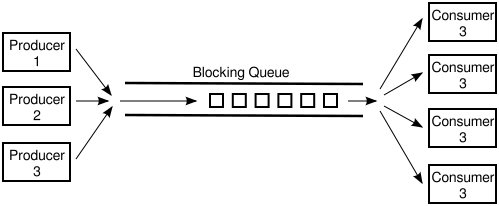
\includegraphics[width=.6\linewidth]{figs/producer-consumer.png}

  \vspace{1em}

  \pause
  \Large \alert{Proč bychom něco takového chtěli dělat?}
  
 %\faWarning \hspace{3pt} Konzument nemůže odebírat data, pokud v zásobníku žádná data nejsou. 

\end{frame}

\begin{frame}
  \frametitle{Producent -- konzument}
  Doimplementujte metody v \texttt{ThreadPool.h} a zajistěte, že
  \begin{enumerate}
    \item Výpočet úloh je paralelní a každá úloha (přidaná pomocí metody \texttt{process}) je zpracována právě jednou (1 bod)
    \item Thread pool nečeká na přidání nových úloh pomocí busy-waitingu \\ 
          (1 bod)
  \end{enumerate}

\end{frame}
}

% Frame with the feedback QR code 
\framefeedback{}

\end{document}
